\documentclass[a4paper, 10pt]{book}
% \usepackage[a4paper, total={6in, 6in}]{geometry}

\usepackage{amssymb}
\usepackage[figuresright]{rotating}

%\usepackage{fontspec}
\usepackage{lmodern}
\usepackage{lipsum}
\usepackage{psl-cover}

% my packages:
\usepackage[utf8]{inputenc}
\usepackage[english]{babel}
\usepackage{amsmath}
\usepackage{amsfonts}
\usepackage{amssymb}
\usepackage{graphicx}
\usepackage{siunitx}
\sisetup{math-micro=\text{µ},text-micro=µ}
\usepackage[euler]{textgreek}
\usepackage{subcaption}
\usepackage{booktabs}
\usepackage{soul}
\usepackage{enumitem}
\usepackage{bm}

\usepackage{notations}

\usepackage{import}
\usepackage{example}
\usepackage{graphicx}
\usepackage{amsmath}
\usepackage{float}
\usepackage{amssymb}
\usepackage{xcolor}
\usepackage{hyperref}
\usepackage{longtable}
\usepackage{listings}
\usepackage{multicol}
\usepackage{import}
\usepackage{comment}
\usepackage{ulem}
\usepackage{booktabs,xltabular}
\usepackage{longtable} 

\title{Insérer ici l'intitulé du sujet de thèse}

\author{Martinus Putra Widjaja}

\institute{MINES ParisTech}
\doctoralschool{Ingénierie des Systèmes, Matériaux, Mécanique, Energétique}{621}
\specialty{Voir spécialités ED}
\date{jj mois aaaa}

%% cotutelle
% \entitle{Thesis Subject in English}
% \otherinstitute{CEA Saclay}
% \logootherinstitute{logo-institute}

\jurymember{1}{Prénom NOM}{Titre, établissement}{Président}
\jurymember{2}{Prénom NOM}{Titre, établissement}{Rapporteur}
\jurymember{3}{Prénom NOM}{Titre, établissement}{Rapporteur}
\jurymember{4}{Prénom NOM}{Titre, établissement}{Examinateur}
\jurymember{5}{Prénom NOM}{Titre, établissement}{Examinateur}
\jurymember{6}{Prénom NOM}{Titre, établissement}{Examinateur}
\jurymember{7}{Prénom NOM}{Titre, établissement}{Examinateur}
\jurymember{8}{Alain THIONNET}{Titre, établissement}{Directeur de thèse}
% \jurymember{9}{Prénom NOM}{Titre, établissement}{Invité}
% \jurymember{10}{Prénom NOM}{Titre, établissement}{Invité}

\frabstract{
  Cuius acerbitati uxor grave accesserat incentivum,
  germanitate Augusti turgida supra modum, quam Hannibaliano
  regi fratris filio antehac Constantinus iunxerat pater,
  Megaera quaedam mortalis, inflammatrix saevientis adsidua,
  humani cruoris avida nihil mitius quam maritus; qui paulatim
  eruditiores facti processu temporis ad nocendum per
  clandestinos versutosque rumigerulos conpertis leviter
  addere quaedam male suetos falsa et placentia sibi
  discentes, adfectati regni vel artium nefandarum calumnias
  insontibus adfligebant.

  Saraceni tamen nec amici nobis umquam nec hostes optandi,
  ultro citroque discursantes quicquid inveniri poterat
  momento temporis parvi vastabant milvorum rapacium similes,
  qui si praedam dispexerint celsius, volatu rapiunt celeri,
  aut nisi impetraverint, non inmorantur.

  Vita est illis semper in fuga uxoresque mercenariae
  conductae ad tempus ex pacto atque, ut sit species
  matrimonii, dotis nomine futura coniunx hastam et
  tabernaculum offert marito, post statum diem si id elegerit
  discessura, et incredibile est quo ardore apud eos in
  venerem uterque solvitur sexus.

  Sed tamen haec cum ita tutius observentur, quidam vigore artuum
  inminuto rogati ad nuptias ubi aurum dextris manibus cavatis
  offertur, inpigre vel usque Spoletium pergunt.\ haec nobilium sunt
  instituta.
}

\enabstract{
  Verum ad istam omnem orationem brevis est defensio. Nam
  quoad aetas M. Caeli dare potuit isti suspicioni locum, fuit
  primum ipsius pudore, deinde etiam patris diligentia
  disciplinaque munita. Qui ut huic virilem togam deditšnihil
  dicam hoc loco de me; tantum sit, quantum vos existimatis;
  hoc dicam, hunc a patre continuo ad me esse deductum; nemo
  hunc M. Caelium in illo aetatis flore vidit nisi aut cum
  patre aut mecum aut in M. Crassi castissima domo, cum
  artibus honestissimis erudiretur.

  Et eodem impetu Domitianum praecipitem per scalas itidem
  funibus constrinxerunt, eosque coniunctos per ampla spatia
  civitatis acri raptavere discursu.\ iamque artuum et
  membrorum divulsa conpage superscandentes corpora mortuorum
  ad ultimam truncata deformitatem velut exsaturati mox
  abiecerunt in flumen.

  Erat autem diritatis eius hoc quoque indicium nec obscurum
  nec latens, quod ludicris cruentis delectabatur et in circo
  sex vel septem aliquotiens vetitis certaminibus pugilum
  vicissim se concidentium perfusorumque sanguine specie ut
  lucratus ingentia laetabatur.

  Ego vero sic intellego, Patres conscripti, nos hoc tempore in
  provinciis decernendis perpetuae pacis habere oportere rationem. Nam
  quis hoc non sentit omnia alia esse nobis vacua ab omni periculo
  atque etiam suspicione belli?
}

\frkeywords{ Caesar licentia post honoratis haec adhibens urbium
  honoratis nullum Caesar.}
\enkeywords{ Delatus delatus nominatus
  onere aut trahebatur quod tenus et bonorum.}

\begin{document}

\maketitle{}

\tableofcontents
\listoffigures


\chapter{Introduction}

\section{Fibre-reinforced composite materials}

\textit{\textbf{general information: fibre-reinforced composites, failure mechanisms, defects, applications; context - pressure vessel safety}} \\

Fibre-reinforced composite materials consist of two phases: fibres and matrix. Fibres are responsible for carrying most loads. In long fibre composites, used in most high performance applications, the behaviour of the composite is highly anisotropic, with stiffness much higher in the fibre direction. Matrix carries part of the loads in the transverse directions, as well as plays a complimentary role under some other loading conditions, for instance controlling the onset of fibre kinking in axial compression. \\

Composite materials can be analyzed at different scales. First, the purely macroscopic structure scale. Secondly, at the level of individual unidirectional plies. Finally, one can consider the properties of the constituents (fibres and matrix) at the microscale. While structure scale is of most interest in engineering practice, it is the microscale phenomena that govern the damage and failure of the material. It is the gap between these two scales that adds complexity to the analysis of composites. \\

\section{Longitudinal tensile failure}

The failure of composites in axial direction is fibre-driven.

\pagebreak
%\clearpage

\section{Plan de la thèse}

\begin{itemize}
\item Introduction
\begin{itemize}
           \item[.] Enjeux et objectifs industriels
           \item[.] L'étude dans le cadre du projet ITN FiBreMod
           \item[.] Objectifs scientifiques et démarche
\end{itemize}

\cite{abbas_hybrid_2018}

\item Les matériaux et les structures envisagés. Mise en évidence des problèmes à résoudre
\begin{itemize}
    \item[.]  Description succinte des structures d'application envisagées
    \item[.]  Description succinte des matériaux envisagés
    \item[.]  Les problèmes de calculs liés à la taille des phénomènes importants au premier ordre sur la rupture des structures
\end{itemize}

\item Rappel de l'existant : modèle de rupture de fibres
\begin{itemize}
    \item[.]  Le modèle existant
    \item[.]  Les validations et les calculs réalisés
    \item[.]  Les problèmes de calculs induits par la taille du phénomène
\end{itemize}

\item Une méthode pour réduire les temps de calcul et la taille des problèmes
\begin{itemize}
           \item[.] Rappel du concept d'ergodicité et du concept de portée intégrale
           \item[.] Application : validation et confirmation de la taille du VER
           \item[.] Application au cas des réservoirs hautes pressions
\end{itemize}

\item Tentative de réduction des temps de calcul et de la taille des problèmes
\begin{itemize}
    \item[.] Un problème de calcul de structure avec l'existant
    \item[.] Un problème de calcul de structure avec l'utilisation de la méthode ergodique
\end{itemize}

\item Calculs et confrontations expérimentales. Mise en place d'un outil de dimensionnement
\begin{itemize}
    \item[.] Cas d'un anneau : expérience et calcul
    \item[.] Cas d'un réservoir : expérience et calcul
    \item[.] Mise en place d'un outil de dimensionnement d'une structure composite à fibres continues
\end{itemize}

\item Conclusion
\begin{itemize}
    \item[.] Synthèse et conclusion de l'étude
    \item[.] Bilan de l'apport de l'étude dans le cadre du projet ITN FiBreMod
    \item[.] Perspectives
\end{itemize}

\end{itemize}


% \chapter{Reference chapter} \label{section_chapter_xxx}


\section{Introduction} \label{section_chapter_xxx_lelabel}

The goal of this study is to establish how a calculation procedure can be developed
which has calculation times and costs acceptable to industrial norms so as to optimise
the design of composite pressure vessels whilst ensuring quantifiable levels of confidences
in their performance. This will be achieved by Finite Element numerical simulation.

The goal of this study is to establish how a calculation procedure can be developed
which has calculation times and costs acceptable to industrial norms so as to optimise
the design of composite pressure vessels whilst ensuring quantifiable levels of confidences
in their performance. This will be achieved by Finite Element \index{Finite Element} numerical simulation.


\section{Exemple de bibliographie} \label{section_chapter_xxx_exemple_de_biblio}

Pour un auteur Batdorf \cite{Batdorf1982a}. Pour deux auteurs Aveston and Kelly \cite{Aveston1973a}.
Pour plus de deux auteurs Aveston {\it et al.} \cite{Aveston1971a}.

\section{Exemple de tableau} \label{section_chapter_xxx_exemple_de_tableau}

Sur le tableau (Tab. \ref{table_chapter_xxx_lelabel}), on voit.
Les resultats montrent la correlation des mesures (Tab. \ref{table_chapter_xxx_lelabel}).


\begin{table}[!ht]
 \begin{center}
    \begin{tabular}{|c|c|c|c|c|c|c|}
   \hline
Cases   & $\gamma$ & $\ln K$ \\
\hline
1D-A  & -0.071 & 10.01 \\
1D-B    & -0.619 & 9.76 \\
1D-C    & -0.596 & 9.73 \\
2D-A    & -0.533 & 10.43 \\
2D-B    & -0.971 & 10.79 \\
2D-C    & -0.591 & 10.69 \\
3D      & -0.820 & 10.86 \\
   \hline
\end{tabular}
    \caption{
    \label{table_chapter_xxx_lelabel}
    Linear Fitting.
    }
 \end{center}
\end{table}


\section{Exemple de figure} \label{section_chapter_xxx_exemple_de_figure}

Sur la figure (Fig. \ref{figure_chapter_xxx_lelabel}), on voit.
Les resultats montrent la correlation des mesures (Fig. \ref{figure_chapter_xxx_lelabel}).

\begin{figure}[!ht]
	\begin{center}
		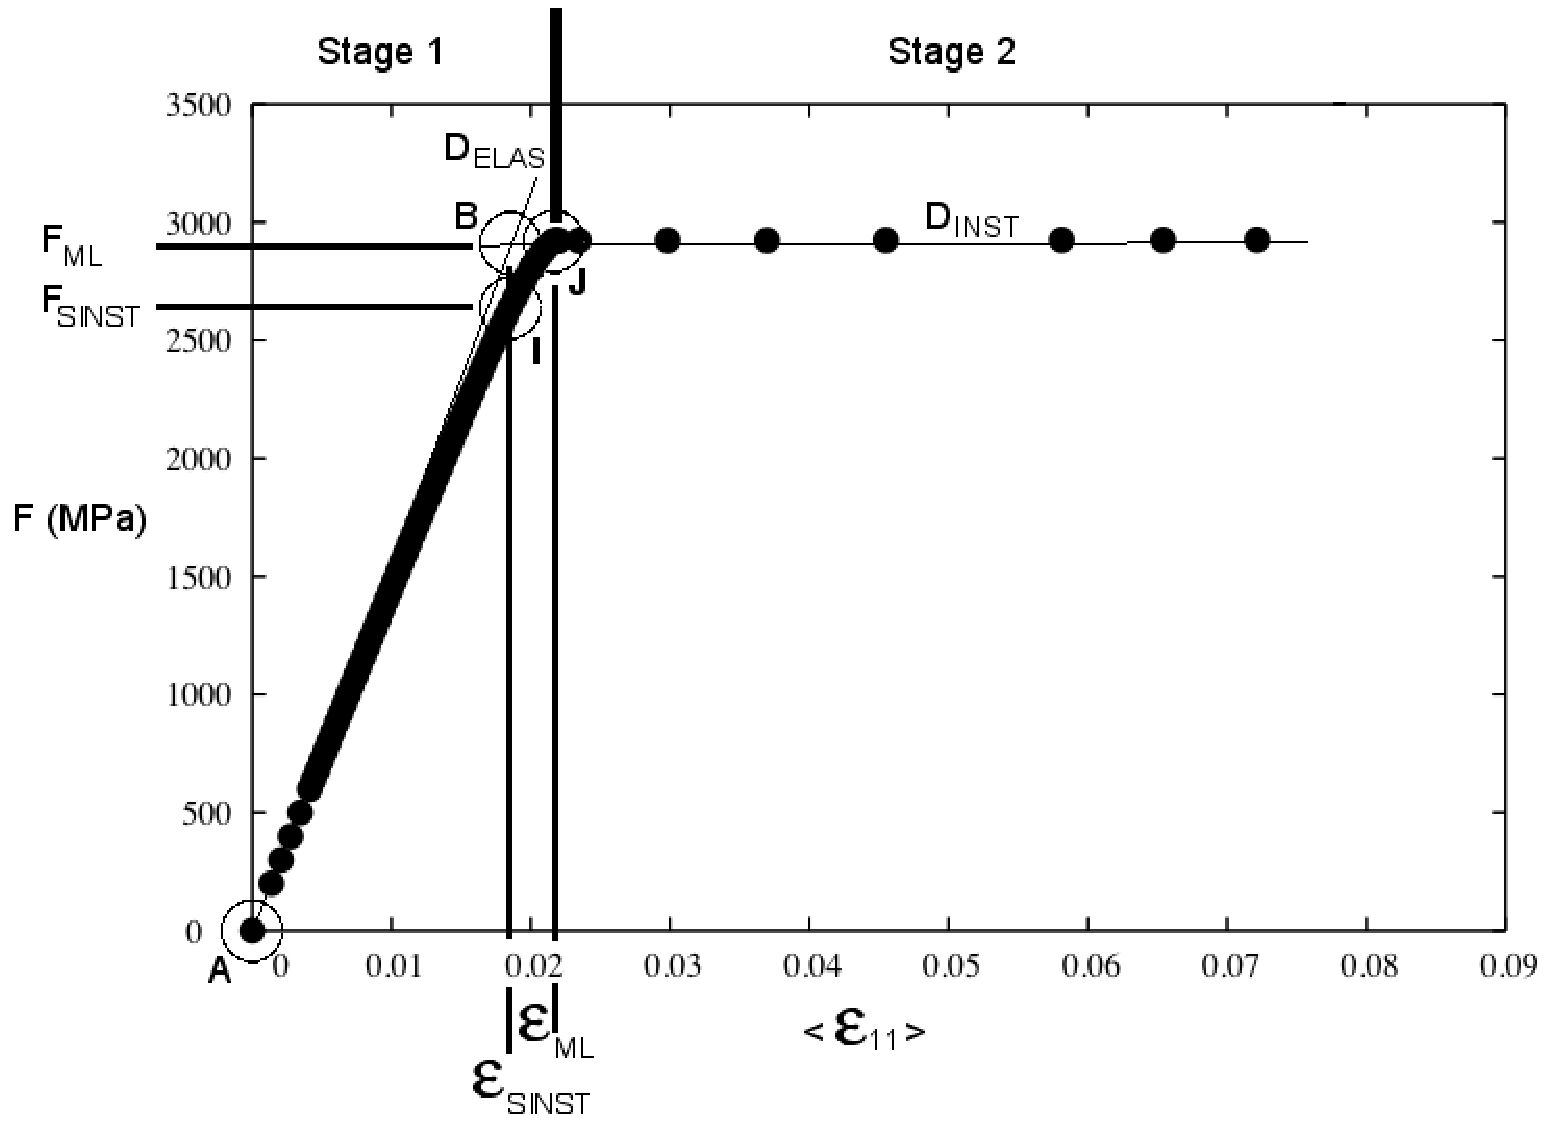
\includegraphics[scale=0.26]{chapters/chapter_model_mise_en_page/figures/figure_1.pdf} \\
		(a) \\
		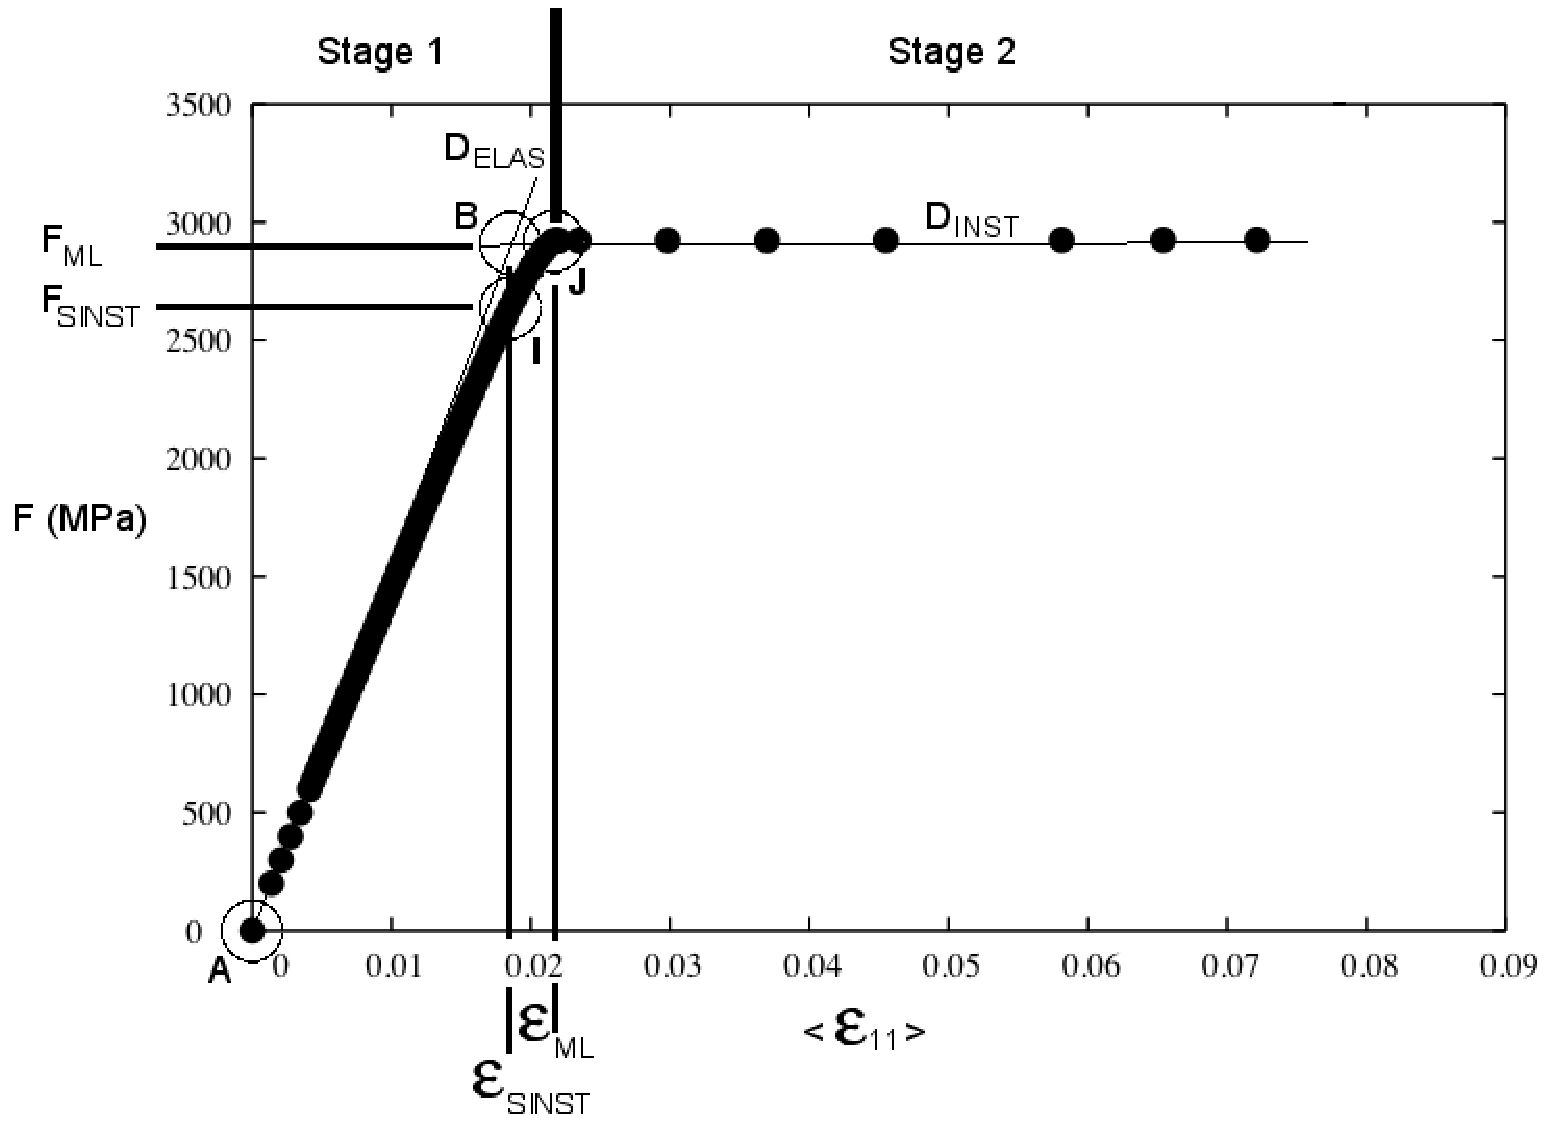
\includegraphics[scale=0.26]{chapters/chapter_model_mise_en_page/figures/figure_1.pdf} \\
		(b)
		\caption{
		\label{figure_chapter_xxx_lelabel}
			Typical loading curves. (a) xxx. (b) yyy.
		}
	\end{center}
\end{figure}

\section{Exemple de formule} \label{section_chapter_xxx_exemple_de_formule}


\begin{equation} \label{equation_chapter_xxx_lelabel}
\begin{split}
{C}^{loc}_{1111}({\cal{V}}(M),{\cal{D}}(M, t))& = V_{f}(M) C_{1111}^{f} (   1 - {\cal{D}}(M, t) )  \\
& + (1-V_{f}(M)) C_{1111}^{m}
\end{split}
\end{equation}






\chapter{Chapter 01}
\label{section_chapter_xxx}

\section{Introduction}
\label{sec_introduction}

\paragraph{Outline}

This paper aims at highlighting the link between the Hu–Washizu
variational principle and that of so called relaxed formulations
% ,
% from which are derived \textit{e.g.} Hybrid Discontinuous Galerkin
% (HDG) methods, and, in particular, one of their latest refinement, the
% Hybrid High Order (HHO) method.
among which the family of Discontinuous Galerkin (DG) and Hybrid Discontinuous Galerkin
(HDG) methods, and, in particular, one of their latest refinement, the
Hybrid High Order (HHO) method.
Both these approaches introduce supplementary unknowns to the problem, and many works in the literature rely on either one of these two approaches to derive numerical methods that prove to be robust to volumetric locking phenomena.
% Both these methods are at the foundation of numerical methods

The Hu-Washizu principle considers supplementary stress and strain fields to the sole displacement problem arising from the well-known principle of Virtual Work, that act as Lagrange multipliers to enforce respectively the constitutive and strain-displacement relations.
On the other hand, relaxed formulations provide a richer kinematics by introducing a displacement jump at element boundaries, hence allowing for the definition of enhanced strain and stress fields.

The present paper proposes a variational formulation for HDG methods based on a Hu-Washizu approach, where the discontinuity of the displacement field is
retrieved by introducing a linear elastic interface between elements, hence sketching a common framework to both Hu-Washizu based approaches for continuous displacement fields, and hybrid discontinuous methods.
An novel resolution algorithm, based on the proposed variational approach is then devised and numerically tested in Section \ref{sec_num_example_part_2}.
Finally, an extension of the method to axi-symmetric problems is proposed.

% The following introduction outlines in a first part the development and applications of The Hu–Washizu variational
% formulation and in a second part that of discontinuous methods.

% DIRE HW A ETE REGARDE POUR LINCOMPRESSIBILITE PLASTIQUE ETC, AVANTDE PARLER DES LETHDODES
% -> INTRODUIRE LES 
% -> NOTATIONS (voir papier micromorphe)
% -> charges mortes pour les temres de passage en configurartion initiale, pas celles de Nanson
% -> les brackets : dimension finie, produit scalair intégrale, nsur des vectiueyrs : produit scalair vectoriel
% -> le potentiel élastique, non-standrad mais pour retrouver les expressions exactes des HDG, passer par vrai potentiel élastique , à tester. Passage en zone cohézive, extension intéressante pas traitée dans le document

% ---------------------------------------------------------
% -- SUBSECTION
% ---------------------------------------------------------
\subsection{From the Hellinger-Reissner principle to the Hu–Washizu variational formulation}

Before 1950, variational principles considered only displacement
as a single independent field.
Generalized variational principles began in the 1950's with the
breakthrough works of Reissner \cite{reissner_variational_1950} on two-field variational principles for elasticity problems, in
which the displacement and stress were considered independent fields. Subsequently, de Vebeuke \cite{fraeijs_de_veubeke_diffusion_1951} constructed a
four-field variational principle, and Hu \cite{hu_variational_1954} and Washizu \cite{washizu_variational_1955} established three-field variational
principle independently.
In 1983, Chien \cite{chien_method_1983} first pointed out that the three kinds of
variables in Hu-Washizu principle are but nct independent
of each other. Stress-strain relations are still its variational
constraints, which could be removed only by high-order
Lagrange multiplier method.

% ---------------------------------------------------------
% -- SUBSUBSECTION
% ---------------------------------------------------------
\paragraph{B-bar methods}

The denomination "assumed strain methods" is intended to encompass a variety of finite element procedures, often proposed on an ad-hoc basis, which are typically characterized by an interpolation of the discrete gradient operator assumed apriori, independently of the interpolation adopted for the displacement field. The often referred to "B-bar method", proposed by Hughes \cite{belytschko_ac0_1984}, offers an example of an assumed strain method which has proven successful in a variety of situations, including widely used structural elements \cite{hughes_finite_1981}. For the finite strain incompressible problem, this method has been precisely reformulated by Simo et al. \cite{simo_variational_1985} within the context of the Hu-Washizu principle.
% The so-called mode decomposition technique, proposed by Belytschko (e.g., [\textcolor{blue}{ref}]), furnishes another example of a B-bar type of method that leads to the formulation of successful structural elements.

% In XXX, Hughes and SImon showed that that assumed strain methods can be systematically formulated within the variational framework furnished by the Hu-Washizu principle. A crucial point in this development concerns the role played by the stress field, now entering the formulation as a Lagrange multiplier, and its recovery within the proposed variational structure. It is first noted that the Lagrange multipliers drop out from the formulation leading to a generalized displacement model, provided a certain orthogonality condition on the assumed strain field is satisfied. In addition, as a result of the variational structure, the admissible stress field (Lagrange multipliers) is constrained by an orthogonality condition arising from the Hu-Washizu principle as an Euler-Lagrange equation. These orthogonality conditions result in a single.

% ---------------------------------------------------------
% PARAGRAPH
% ---------------------------------------------------------
\paragraph{Mixed methods}

At the same time,
studies concerning the equivalence of the modified displacement approaches and Hu-Washizu
mixed approaches were conducted by Simo et al. \cite{simo_variational_1985} with regard to incompressibility
problems, and by Simo and Hughes \cite{simo_variational_1985} in a more general context of the assumed strain
(B-bar) approach. Other related works are \cite{hughes_equivalence_1977,oden_observations_1975, shimodaira_equivalence_1985}

% ---------------------------------------------------------
% -- SUBSECTION
% ---------------------------------------------------------
\subsection{Hybrid Discontinuous Galerkin methods}

% The Hybrid High Order method (HHO) is a discontinuous discretization
% method, that takes root in the Discontinuous Galerkin method (DG).
From the physical standpoint, discontinuous methods ensure the continuity of the flux
across interfaces, by seeking the solution element-wise, hence allowing
jumps of the potential across elements. They can be seen as a
generalization of Finite Volume methods, and are able to capture
physically relevant discontinuities without producing spurious
oscillations.

% ---------------------------------------------------------
% -- SUBSUBSECTION
% ---------------------------------------------------------
\paragraph{Discontinuous Galerkin (DG) methods}

The origin of DG methods dates back to the pioneering work of
\cite{reed_triangular_1973}, where an hyperbolic formualtion is used to
solve the neutron transport equation. The first application of the
method to elliptic problems originates in \cite{babuska_finite_1973}
where Nitsche's method \cite{nitsche_uber_1970} is used to weakly impose
continuity of the flux across interfaces.

% ---------------------------------------------------------
% PARAGRAPH
% ---------------------------------------------------------
\paragraph{Application in Linear Elasticity}

% ---> TODO : reformulate
In 2002, Hansbo and Larson \cite{hansbo_discontinuous_2002-1} were the first to
consider the Nitsche's classical DG method for nearly incompressible
elasticity. They showed, theoretically and numerically, that this
method is free from volumetric locking.
% --->
%
%

% ---------------------------------------------------------
% PARAGRAPH
% ---------------------------------------------------------
\paragraph{Symmetric interior penalty}

However, the bilinear form
arising from this formulation is not symmetric. A so called interior
penalty term has been introduced in \cite{wheeler_elliptic_1978},
leading to the Symmetric Interior Penalty (SIP) DG method. A first study
of the method to linear elasticity has been devised by
\cite{riviere_optimal_2000}, where optimal error estimate has been
proved.
%
%
%
% ---> TODO : reformulate
\cite{lew_optimal_2004} generalized the
Symmetric Interior Penalty method to linear elasticity.
In about the same
period of time, DG methods were proposed for other linear problems in
solid mechanics, such as Timoshenko beams
\cite{celiker_locking-free_2006}, Bernoulli-Euler beam and the
Poisson-Kirchhoff plate \cite{brenner_balancing_1999,
  engel_continuousdiscontinuous_2002} and Reissner-Mindlin plates
\cite{arnold_family_2005}. In the mid 2000's, the first applications
of DG methods to nonlinear elasticity problems was undertaken by
\cite{ten_eyck_discontinuous_2006, noels_general_2006}, and in 2007,
Ortner and Süli \cite{ortner_discontinuous_2007} carried out the a
priori error analysis of DG methods for nonlinear elasticity.
% --->

% ---------------------------------------------------------
% PARAGRAPH
% ---------------------------------------------------------
\paragraph{DG methods in solid mechanics}
%
%
%
DG methods then sollicitated a vigourus interest, mostly in fluid dynamics \cite{shahbazi_high-order_2007, persson_discontinuous_2009} due to their local conservative property and stability in convection domniated problems. However, except some applications for instance in fracture mechanics using XFEM methods \cite{gracie_blending_2008, shen_stability_2010}, or gradient plasticity \cite{djoko_discontinuous_2007,djoko_discontinuous_2007-1} DG methods did not break through in computational solid mechanics because of their numerical cost, since nodal unknowns need be duplicated to define local basis functions in each element.

% ---------------------------------------------------------
% -- SUBSUBSECTION
% ---------------------------------------------------------
\paragraph{Hybrid Discontinuous Galerkin (HDG) methods}

To adress this problem, in the early 2010's, \cite{cockburn_unified_2009, soon_hybridizable_2009} introduced additional faces unknowns on element interfaces for linear elastic problem, hence leading to the hybridization of DG methods, or Hybridizable Discontinuous Galerkin method (HDG). By adding supplementary boundary unknowns, the authors actually allowed to eliminate original cell unknowns by a static condensation process, in order to express the global problem on faces ones only.

% ---------------------------------------------------------
% PARAGRAPH
% ---------------------------------------------------------
\paragraph{HDG methods in solid mechanics}

Extension of HDG methods to non-linear elasticity were first undertaken in \cite{soon_hybridizable_2008} and have then fueled intense reaserch works for various applications such as linear and non-linear convection-diffusion problems \cite{nguyen_implicit_2009,nguyen_implicit_2009-1,nguyen_hybridizable_2010}, incompressible stokes flows \cite{nguyen_hybridizable_2010, nguyen_implicit_2011} and non-linear mechanics \cite{nguyen_hybridizable_2012}.

% ---------------------------------------------------------
% PARAGRAPH
% ---------------------------------------------------------
\paragraph{HHO methods}

In \cite{di_pietro_hybrid_2015, di_pietro_arbitrary-order_2014}, the authors introduced a higher order potential reconstruction operator in the classical HDG formulation for elliptic problems, providing a $h^{k+1} H^1$-norm convergence rate as compared to the ususal $h^k$-rate. This higher order term coined the name for the so called HHO method.
Recent developments of HHO methods in
computational mechanics include the incompressible Stokes
equations (with possibly large irrotational forces) \cite{di_pietro_discontinuous_2016}, the
incompressible Navier–Stokes equations \cite{di_pietro_hybrid_2018}, Biot’s consolidation problem \cite{boffi_nonconforming_2016}, and nonlinear elasticity with small
deformations \cite{botti_hybrid_2017}

% \subsection{Aim of this paper}

% \subsection{Outline}

% In the first part of this paper, the Hu-Washizu variational principle is presented, and the Principle of Virtual Work is introduced as specification of the Hu-Washizu principle.
% The description of an element 
% ---------------------------------------------------------
% ---- SECTION
% ---------------------------------------------------------
\section{The standard Hu–Washizu variational approach}
\label{sec_model_problem}

This section introduces the standard Hu–Washizu three field
principle. For the sake of simplicity, and without loss of generality,
let consider the case of an hyperelastic material. Extensions to
mechanical behaviours with internal state variables are treated in
classical textbooks of computational mechanics
\cite{belytschko_nonlinear_nodate,besson_non-linear_2010}. This
extension in
Section~\ref{sec:discretization:extension_to_non_linear_materials} for
theorical aspects and in Section~\ref{sec_implementation} which
discusses our numerical implementation of the Hybrid High Order method.
This implementation is used in Section~\ref{sec_numerical_examples}
which provides several examples in finite strain plasticity.

% ---------------------------------------------------------
% -- SUBSECTION
% ---------------------------------------------------------
\subsection{Description of the mechanical problem and notations}

% ---------------------------------------------------------
% PARAGRAPH
% ---------------------------------------------------------
\paragraph{Solid body}

Let us consider a solid body whose reference configuration is denoted
$\bodyLag$. At a given time $t > 0$, the body is in the current
configuration $\bodyEul$.

% ---------------------------------------------------------
% PARAGRAPH
% ---------------------------------------------------------
\paragraph{Mechanical loading}

The body is assumed to be submitted to a body force $\loadEul$ acting
in $\bodyEul$, a prescribed displacement $\dirichletEul$ on the
Dirichlet boundary $\dirichletBoundaryEul$, and a contact load
$\neumannEul{}$ on the Neumann boundary $\neumannBoundaryEul$.

% ---------------------------------------------------------
% PARAGRAPH
% ---------------------------------------------------------
\paragraph{Deformation}

The transformation mapping 
$\tensori{\Phi}$ takes a point from the reference configuration $\bodyLag$ to the current
configuration $\bodyEul$ such that
%
%
%
\begin{equation}
    \tensori{\Phi}\paren{\tensori{X}} = \tensori{x} = \tensori{X}+\tensori{u}\paren{\tensori{X}}
\end{equation}
%
%
%
where $\tensori{X}$, $\tensori{x}$ and $\tensori{u}$ denote respectively
the position in the reference configuration $\bodyLag$, the position
in the current configuration $\bodyEul$ and the displacement.

% ---------------------------------------------------------
% PARAGRAPH
% ---------------------------------------------------------
\paragraph{Deformation gradient, gradient of the displacement}

The deformation gradient $\tensorii{F}$ is defined as
%
%
%
\begin{equation}
    \tensorii{F} = \nabla \tensori{\Phi} = \tensorii{I} + \tensorii{G}
\end{equation}
%
%
%
where $\nabla$ is the gradient operator in the
reference configuration and 
%
%
%
\begin{equation}
    \label{eq_grad_def}
    \tensorii{G} = \nabla \tensori{u}
\end{equation}
%
%
%
denotes the gradient of the
displacement.

% ---------------------------------------------------------
% PARAGRAPH
% ---------------------------------------------------------
\paragraph{Stress tensor}

The body is assumed made of an hyperelastic material described by a
free energy $\mecPotential_{\bodyLag{}}$ which relates the deformation gradient
$\tensorii{F}$ and the first Piola-Kirchhoff stress tensor $\tensorii{P}$ such that
%
%
%
\begin{equation}
    \label{eq_stress_def}
\tensorii{P}=\deriv{\mecPotential_{\bodyLag{}}}{\tensorii{F}}
\end{equation}

% ---------------------------------------------------------
% -- SUBSECTION
% ---------------------------------------------------------
\subsection{Primal problem and Principle of Virtual Work}

% ---------------------------------------------------------
% PARAGRAPH
% ---------------------------------------------------------
\paragraph{Total lagrangian}

The total Lagrangian $L^{VW}_{\bodyLag{}}$ of the body is defined as
the stored energy minus the work of external loadings, as follows:
%
%
%
\begin{equation}
\label{eq_Lagrangian}
L^{VW}_{\bodyLag{}}
% \paren{\tensori{u}}
= \int_{\Omega}\mecPotential_{\bodyLag{}}
(\tensorii{F}(\tensori{u}))
% \paren{\tensorii{F}\paren{\tensori{u}}}
- \int_{\bodyLag} \tensori{f}{}_V \cdot \tensori{u}{}
- \int_{\neumannBoundaryLag} \neumannLag{} \cdot \tensori{u}{}
\vert_{\neumannBoundaryLag}
\end{equation}
%
%
%
where the body forces $\tensori{f}_{V}$ and conctat tractions
$\neumannLag$ in the reference configuration have been obtained from
their counterparts $\tensori{f}_{v}$ and $\neumannEul$ using the
Nanson formulae,
and where the displacement field is prescribed by $\dirichletLag$ on $\dirichletBoundaryLag{}$ in the reference configuration.
In the following, Dirichlet boundary conditions are omitted from the developments for conciseness.
Moreover, the volumetric and surface load loadings are

% ---------------------------------------------------------
% PARAGRAPH
% ---------------------------------------------------------
\paragraph{Principle of Virtual Works}

The displacement $\tensori{u}$ satisfying
the mechanical equilibrium minimizes the Lagragian $L^{VW}_{\bodyLag{}}$.
The first order variation of Lagrangian is given by
%
%
%
\begin{equation}
  \label{eq_virtual_works_0}
  \frac{\partial L^{VW}_{\bodyLag{}}
    % \paren{\tensori{u}}
  }{\partial \tensori{u}} \cdot \delta \tensori{u} =
  \int_{\bodyLag} \tensorii{P} : \nabla \delta \tensori{u} -
  \int_{\bodyLag} \tensori{f}_V \cdot \delta \tensori{u} -
  \int_{\neumannBoundaryLag} \neumannLag{} \cdot \delta \tensori{u}
  \vert_{\neumannBoundaryLag}
\end{equation}
%
%
%
which must be null for the the solution displacement. The solution
displacement thus satisfies the principle of virtual work
%
%
%
\[
\int_{\bodyLag} \tensorii{P} : \nabla \delta \tensori{u} =
\int_{\bodyLag} \tensori{f}_V \cdot \delta \tensori{u} +
\int_{\neumannBoundaryLag} \neumannLag{} \cdot \delta \tensori{u}
\vert_{\neumannBoundaryLag}
\quad
\forall \delta \tensori{u}{}
\]

% ---------------------------------------------------------
% -- SUBSECTION
% ---------------------------------------------------------
\subsection{The Hu-Washizu Lagrangian}
\label{sec_HW_lagrangian}

The Hu-Washizu Lagrangian $L^{HW}_{\bodyLag{}}$
\cite{belytschko_nonlinear_nodate,washizu_variational_1974} generalizes
the previous variational principle by considering that the gradient of
the displacement $\tensorii{G}$ and the first Piola-Kirchoff
$\tensorii{P}$ stress are independent unknowns of the problem, such
that:
%
%
%
\begin{equation}
  \label{eq_HW_0} L^{HW}_{\bodyLag{}}
  % \paren{\tensori{u},\tensorii{G}, \tensorii{P}}
  = \int_{\bodyLag{}}
  \mecPotential_{\bodyLag{}} (\tensorii{I}+\tensorii{G} ) + (\nabla
  \tensori{u}{} - \tensorii{G}{})\,\colon\,\tensorii{P} -
  \int_{\bodyLag{}} \loadLag \cdot \tensori{u}{} -
  \int_{\neumannBoundaryLag{}} \neumannLag{} \cdot \tensori{u}
  \vert_{\neumannBoundaryLag}
\end{equation}
%
%
%
The solution $(\tensori{u}, \tensorii{G}, \tensorii{P})$
satisfying the mechanical equilibrium minimizes the Lagragian
$L^{HW}_{\bodyLag{}}$. The first order variation of the Hu-Washizu
Lagragian with respect to $\tensori{u}, \tensorii{G}$, and
$\tensorii{P}$ yields % % %
\begin{subequations}
  \label{eq_hu_washizu_derivative_0}
  \begin{alignat}{3}
    \deriv{L^{HW}_{\bodyLag{}}}{\tensori{u}}
    \cdot \delta \tensori{u} = & \int_{\bodyLag} \tensorii{P} : \nabla
    \delta \tensori{u} - \int_{\bodyLag} \tensori{f}_V \cdot \delta
    \tensori{u} - \int_{\neumannBoundaryLag} \neumannLag \cdot \delta
    \tensori{u} \vert_{\neumannBoundaryLag} && \ \ \ \ \ \ \ \ &&
    \forall \delta \tensori{u}{} \label{eq_hu_washizu_derivative_0:eq0}
    \\
    \deriv{L^{HW}_{\bodyLag{}}}{\tensorii{P}}
    : \delta \tensorii{P} = & \int_{\bodyLag} ( \nabla \tensori{u} -
    \tensorii{G} ) : \delta \tensorii{P} && \ \ \ \ \ \ \ \ && \forall
    \delta \tensorii{P}{} \label{eq_hu_washizu_derivative_0:eq2} \\
    \deriv{L^{HW}_{\bodyLag{}}}{\tensorii{G}}
    : \delta \tensorii{G} = & \int_{\bodyLag} (\frac{\partial
      \mecPotential}{\partial \tensorii{G}} - \tensorii{P}) : \delta
    \tensorii{G} && \ \ \ \ \ \ \ \ && \forall \delta \tensorii{G}{}
    \label{eq_hu_washizu_derivative_0:eq3}
  \end{alignat}
\end{subequations}
where Equations~\eqref{eq_hu_washizu_derivative_0:eq2}
and~\eqref{eq_hu_washizu_derivative_0:eq3} account
for~\eqref{eq_grad_def} and~\eqref{eq_stress_def} respectively in a weak
sense.

% ---------------------------------------------------------
% -- SUBSECTION
% ---------------------------------------------------------
\subsection{Classical applications of the Hu-Washizu variational
  approach in computational mechanics to circumvent volumetric locking}

In the continuous framework, the Hu-Washizu functional is not
relevant, since Equations~\eqref{eq_hu_washizu_derivative_0:eq2}
and~\eqref{eq_hu_washizu_derivative_0:eq3} would lead to the following
egualities:
%
%
%
\begin{equation}
  \begin{aligned}
    \tensorii{G} = \nabla\tensori{u} && \text{and} && \tensorii{P}=\frac{\partial \mecPotential}{\partial \tensorii{G}}
  \end{aligned}
\end{equation}
%
%
%
% \[
% \tensorii{G} = \nabla\tensori{u}
% \quad\text{and}\quad
% \tensorii{P}=\frac{\partial \mecPotential}{\partial \tensorii{G}}
% \]
% 
However, considering finite-dimensional functional spaces, multiple choices arise
for the specification of the Lagrangian \eqref{eq_HW_0}.

% ---------------------------------------------------------
% PARAGRAPH
% ---------------------------------------------------------
\paragraph{Pressure swelling formulations}

Since volumetric locking is a pressure dependent phenomenon,
considering for instance a decomposition of the stress and strain fields
into \textit{e.g.} devatoric and spherical components, one can express a
mixed problem in terms of pressure and swelling, which is at the origin
of so-called UPG methods \cite{al_akhrass_integrating_2014,
  simo_quasi-incompressible_1991,simo_variational_1985}. The scalar
pressure and swelling unknowns replace respectively the stress and
strain tensorial unknowns in \eqref{eq_HW_0} and a modified deformation
gradient is introduced in the constitutive equation.

% ---------------------------------------------------------
% -- SUBSECTION
% ---------------------------------------------------------
\paragraph{Enhanced assumed strains formulations}

Another approach of the use of the Hu-Washizu consists in
studying the equilibrium of a single element. Such a framework falls
into the scope of so-called Enhanced Assumed Strains methods
\cite{simo_variational_1986,simo_class_1990}, which results for instance
in the B-bar method, that consists in defining a modified derivation
operator, such that one gets rid of the three-field formulation, to
express the problem in terms of primal unknowns only.

% ---------------------------------------------------------
% -- SUBSECTION
% ---------------------------------------------------------
\paragraph{Towards Discontinuous methods}

In the present document, we propose an introduction to so-called
\textit{non-conformal} methods, by means of the Hu–Washizu Lagrangian.
At the origin of these methods is the Discontinuous Galerkin (DG)
method, which postulates the discontinuity of the displacement across
elements. This feature allows the method to be robust to volumetric
locking. However, its formulation takes root in a possibly dry
mathematical background, and the ingredients of the method are not
introduced in the literature through physical arguments. The goal of the
next section aims at introducing the whole framework of non-conformal
methods, including the displacement discontinuity, through the
Hu–Washizu Lagragian.

% In \cite{noels_general_2006,neunteufel_three-field_2021}, a Hu-Washizu Lagrangian is used in the context of discontinuous methods (namely the DG and the TDNNS methods), but it does not account for the global framework defining these methods, as in the present document.

% Though one counts a few occurances of the use of the Hu–Washizu Lagragian in the context of discontinuous methods \cite{noels_general_2006,neunteufel_three-field_2021}, none, to our knowledge, introduce all the ingredients of the method through the 
% sole Hu–Washizu Lagragian.

% and though one counts a few applications of the Hu–Washizu Lagrangian for Discontinuous Galerkin methods \cite{}, none of them exploit the 
% Its application in mechanics had not resulted in a break through, and
% so did not its variants, among which the Hybird Discontinuous Galerkin method and the Hybird High Order method.
% Though one counts a few applications of the Hu–Washizu Lagrangian for Discontinuous Galerkin methods 

% En continue, aucun intérêt. Par contre, très puissant une fois les
% bases d'approximations choisies.

% Many variants:

% - Ne considérer uniquement l'espace sphérique.

% - Gardez des champs globaux: U-P-G inconnues nodales. Variantes liées aux choix des espaces d'approximations de U, P et G (Al-Akrass).

% - Travailler par éléments: Assumed strain (c.f. Belytchko).

% ---------------------------------------------------------
% ---- SECTION
% ---------------------------------------------------------
\section{Introduction to the Hybrid Discontinuous Galerkin methods through the Hu-Washizu variational principle}
\label{sec_composite_demo}

In this section, let $\cell$ a subpart, called cell in the rest of the
text, of the body \(\bodyLag\). In the following, one assumes that the
cell $\cell$ is located inside the body $\bodyLag{}$, such that its
boundary $\dCell{}$ bears contact loads only. This subpart is in
equilibrium with the rest of the body \(\Omega\backslash T\) if the
displacements and the normal traction are continuous at the boundary
$\dCell{}$.

% ---------------------------------------------------------
% PARAGRAPH
% ---------------------------------------------------------
\paragraph{Conformal methods} Enforcing the displacement continuity at the interface leads to
so-called conformal methods, to which the standard Finite Element (FE), or Lagrange
method belongs (see Figure \ref{fig_02}(a)).

% ---------------------------------------------------------
% PARAGRAPH
% ---------------------------------------------------------
\paragraph{Discontinuous Galerkin methods} On
the contrary, this condition can be weakened by introducting an elastic
interface of negligible size between \(T\) and \(\Omega\backslash T\).
This representation is at the basis of Discontinuous Galerkin methods
(see Figure \ref{fig_02}(b)).

% ---------------------------------------------------------
% PARAGRAPH
% ---------------------------------------------------------
\paragraph{Hybird Discontinuous Galerkin methods} In
this paper, we consider hybrid discontinuous Galerkin (HDG) methods,
where two elastic interfaces are introducted: one between \(T\) and its
boundary \(\partial T\) and a second one between \(\Omega\backslash T\)
and \(\partial T\) (see Figure \ref{fig_02}(c)). Following this idea, we
show in this section how the use of the Hu-Hashizu Lagrangian allows to
recover the main ingredients of the HDG/HHO methods, namely the
\textit{reconstructed gradient} and the \textit{stabilisation operator}.

% ---------------------------------------------------------
% -- SUBSECTION
% ---------------------------------------------------------
\subsection{Element description}

% ---------------------------------------------------------
% PARAGRAPH
% ---------------------------------------------------------
\paragraph{Element geometry}

In the following, the cell $\cell$ is assumed to be convex.
It is split into a core part $\Bulk \subset \cell$ with boundary $\dBulk$, and into an interface part $\Crown{} \subset \cell$ with boundary $\dCrown = \dBulk \cup \dCell$, as shown in Figure \ref{fig_02}. The interface $\Crown{}$ has some thickness $\ell > 0$ that is supposed to be small compared to $h_{\cell}$ the diameter of $\cell$.
From a geometrical standpoint, the core par of the element $\Bulk{}$ is an homotethy of $\cell$ by some ratio inferior to $1$.

% ---------------------------------------------------------
% PARAGRAPH
% ---------------------------------------------------------
\paragraph{Element boundary description} The boundary $\dCell{}$ of $\cell$ is the composition of a Neumann boundary $\neumannCell{}$ and a Dirichlet $\dirichletCell{}$, if the element $\cell$ shares a boundary with $\dirichletBoundaryLag{}$. In the following, for the sake of simplicity, we assume that the element is located inside the body $\bodyLag{}$, such that is only subjected to imposed traction forces on $\neumannCell{} = \dCell{}$ with $\dirichletCell{} = \emptyset$.
%
% 
% 
\begin{figure}[H]
    \centering
    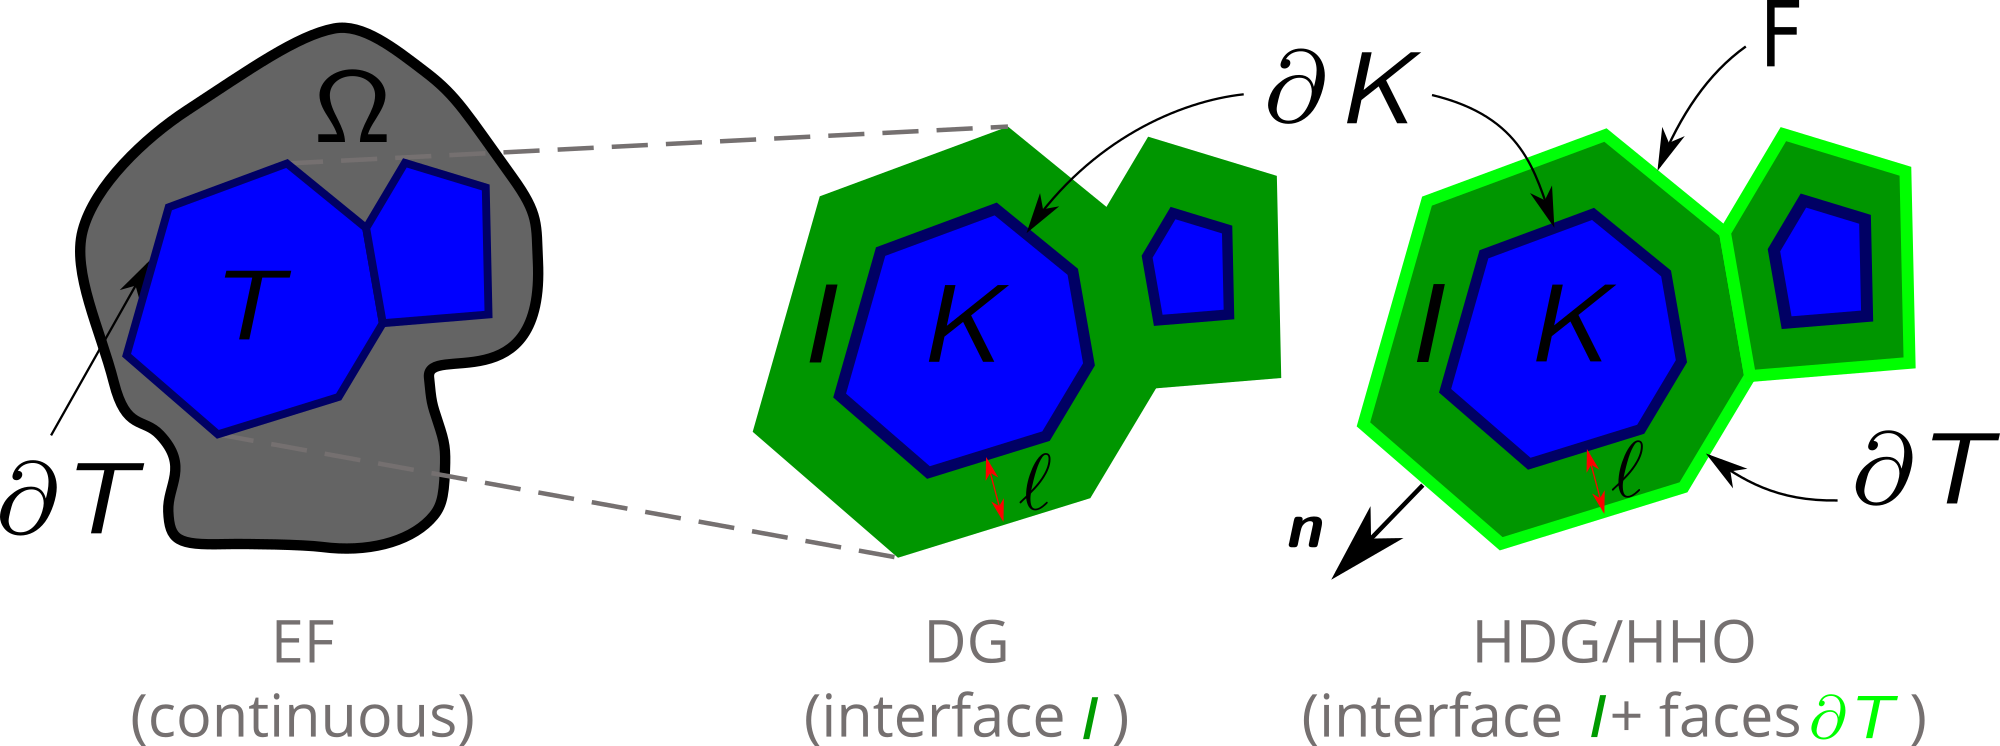
\includegraphics[width=14.cm]{img_calcs/ef_dg_hdg.png}
    \caption{schematic representation of a cell and its surrounding depending on the continuity requirement of the displacement field}
    \label{fig_02}
\end{figure}
%
%
%

% ---------------------------------------------------------
% PARAGRAPH
% ---------------------------------------------------------
\paragraph{Element behaviour}

The core of the element $\Bulk{}$ is made out of the same material that composes $\Omega$ and behaves according to the free energy potential $\mecPotential{}_{\bodyLag{}}$. The interface $\Crown{}$ is made out of a pseudo linear elastic material of Young modulus $\beta (\ell / h_{\cell})$ with a zero Poisson ratio and its behavior is defined by the free energy potential $\mecPotential{}_{\Crown{}}$ such that
%
%
%
\begin{equation}
    \label{eq_0009}
        \mecPotential{}_{\Crown} = \frac{1}{2} \beta \frac{\ell}{h_{\cell}} \nabla \tensori{u}{}_{\Crown} : \nabla \tensori{u}{}_{\Crown}
\end{equation}
%
%
%
where the dimensionless ratio $\ell / h_{\cell}$ balances the accumulated energy with the size of the domain $\cell$.

% ---------------------------------------------------------
% PARAGRAPH
% ---------------------------------------------------------
\paragraph{Element loading}

The core $\Bulk$ is subjected to the volumetric loading $\loadLag{}$, and to the traction force applied by the interface $\Crown{}$ onto $\dBulk{}$. By continuity, $\Bulk{}$ applies the opposite traction force on $\Crown{}$ through $\dBulk{}$. The interface $\Crown{}$ is also subjected to the exterior traction force $\neumannCellLoad{}$ acting on $\neumannCell{}$, that accounts for the action of the rest of the solid $\bodyLag{}$ onto the boundary $\dCell$.

% ---------------------------------------------------------
% PARAGRAPH
% ---------------------------------------------------------
\paragraph{Discplacement, displacement gradient and stress fields}

Let note $\tensori{u}{}_{\Bulk}$ the displacement field, $\tensorii{G}{}_{\Bulk}$ the displacement gradient field and $\tensorii{P}{}_{\Bulk}$ the stress field in $\Bulk{}$. Similarly, let $\tensori{u}{}_{\Crown{}}$ the displacement field, $\tensorii{G}{}_{\Crown}$ the displacement gradient field and $\tensorii{P}{}_{\Crown}$ the stress field in $\Crown{}$.
The displacement of the boundary $\dCell{}$ is denoted $\tensori{u}{}_{\dCell{}}$.
By continuity of the displacement field between $\Bulk{}$ and $\dCell$,  the displacement $\tensori{u}{}_{\Crown{}}$ verifies
%
% 
% 
\begin{subequations}
    \label{eq_conformity}
        \begin{alignat}{2}
        \tensori{u}{}_{\Crown} \vert_{\dBulk} & = \tensori{u}{}_{\Bulk} \vert_{\dBulk}
        \label{eq_conformity:eq1}
        \\
        \tensori{u}{}_{\Crown} \vert_{\dCell} & = \tensori{u}{}_{\dCell}
        \label{eq_conformity:eq2}
    \end{alignat}
\end{subequations}

% ---------------------------------------------------------
% PARAGRAPH
% ---------------------------------------------------------
\paragraph{Hu-Washizu Lagrangian of the element}

By combining both the Lagragian of the core $\Bulk{}$ and that of the interface $\Crown{}$, one obtains the total Lagragian $L_{\cell}^{HW}$ over the element such that
%
%
%
\begin{equation}
    \label{eq_hu_washizu_split}
    L_{\cell}^{HW}
    % (\tensori{u}{}_{\cell}, \tensorii{G}{}_{\cell}, \tensorii{P}{}_{\cell})
    =
    \int_{\Bulk} \mecPotential_{\bodyLag{}} + (\nabla \tensori{u}{}_{\Bulk} - \tensorii{G}{}_{\Bulk}) : \tensorii{P}{}_{\Bulk}
    +
    \int_{\Crown} \mecPotential_{\Crown{}} + (\nabla \tensori{u}{}_{\Crown} - \tensorii{G}{}_{\Crown}) : \tensorii{P}{}_{\Crown}
    -
    \int_{\Bulk} \loadLag \cdot \tensori{u}{}_{\Bulk}
    % -
    % \int_{\Crown} \loadLag \cdot \tensori{u}{}_{\Crown}
    -
    \int_{\neumannCell} \neumannCellLoad \cdot \tensori{u}{}_{\dCell}
\end{equation}

% ---------------------------------------------------------
% -- SUBSECTION
% ---------------------------------------------------------
\subsection{Hypotheses}
\label{sec_assumtions}

Since the interface is of negligible volume compared to that of the core, let make the following assumptions on the displacement and the stress fields in the interface.

% ---------------------------------------------------------
% PARAGRAPH
% ---------------------------------------------------------
\paragraph{Displacement in the interface}

The displacement in the interface $\Crown$ is assumed to be linear with respect to $\tensori{n}$, such that
its gradient is homogeneous in $\Crown{}$ along $\tensori{n}$
%
% 
% 
\begin{equation}
    \label{eq_crown_displacement}
    \nabla
    \tensori{u}{}_{\Crown}
    =
    \frac{\tensori{u}{}_{\dCell}
    -
    \tensori{u}{}_{\Bulk} \vert_{\dBulk} }{\ell} \otimes \tensori{n}
\end{equation}
% 
% 
%
That is, the displacement of the interface $\Crown{}$ linearly bridges that of the boundary $\dCell{}$ to that of the bulk $\Bulk{}$.

% ---------------------------------------------------------
% PARAGRAPH
% ---------------------------------------------------------
\paragraph{Stress in the interface}

Furthermore, let assume that $\tensorii{P}{}_{\Crown}$ is constant along the direction $\tensori{n}{}$ in $\Crown{}$. By continuity of the traction force across $\dBulk$, the following equality holds true
%
% 
% 
\begin{equation}
    \label{eq_continuity_traction_force}
    \begin{aligned}
        (\tensorii{P}{}_{\Crown} \vert_{\dBulk{}} - \tensorii{P}{}_{\Bulk} \vert_{\dBulk{}}) \cdot \tensori{n}{} = 0
        % &&
        % \text{in}
        % &&
        % \Crown{}
    \end{aligned}
\end{equation}

% ---------------------------------------------------------
% -- SUBSECTION
% ---------------------------------------------------------
\subsection{Towards Hybrid discontinuous methods from the Hu-Washizu Lagrangian}

Using the hypotheses stated in Section \ref{sec_assumtions} on the displacement field and the stress field in $\Crown{}$,
one can write \eqref{eq_hu_washizu_split} as a term depending on the thickness of the interface $\ell$ and on the core and boundary unknowns only. The reader can refer to \ref{sec_appendix_Hu_Washizu} for more details.

% ---------------------------------------------------------
% PARAGRAPH
% ---------------------------------------------------------
\paragraph{Simplified Hu–Washizu Lagrangian for a vanishing interface}

In particular, making the thickness of the interface $\ell \rightarrow 0$, such that $\Crown{}$ vanishes and the core part $\Bulk{}$ identifies to $\cell$, one obtains the simplified Hu–Washizu Lagrangian
% 
% 
%
\begin{equation}
    \label{eq_0015}
    \begin{aligned}
        L_{\cell}^{HW}
        = &
        \int_{\cell{}} \mecPotential{}_{\bodyLag{}} + (\nabla \tensori{u}{}_{\cell{}} - \tensorii{G}{}_{\cell{}}) : \tensorii{P}{}_{\cell}
        % \\
        % &
        + \int_{\dCell{}} (\tensori{u}{}_{\dCell} - \tensori{u}{}_{\cell} \vert_{\dCell}) \cdot \tensorii{P}{}_{\cell} \vert_{\dCell{}} \cdot \tensori{n}{}
        % \\
        % &
        + \int_{\dCell} \frac{\beta}{2 h_{\cell}} \lVert \tensori{u}{}_{\dCell{}} - \tensori{u}{}_{\cell{}} \vert_{\dCell{}} \rVert^2
        \\
        &
        -
        \int_{\cell} \loadLag{} \cdot \tensori{u}{}_{\cell{}}
        -
        \int_{\neumannCell{}} \neumannCellLoad{} \cdot \tensori{u}{}_{\dCell{}}
    \end{aligned}
\end{equation}
%
%
%
which fully defines the equilibrium of an element for discontinuous methods.

% ---------------------------------------------------------
% PARAGRAPH
% ---------------------------------------------------------
\paragraph{Hybridization of the primal unknown; the HDG and HHO methods}

Since the interface $\Crown{}$ has vanished by making $\ell \rightarrow 0$, both $\tensori{u}{}_{\cell} \vert_{\dCell{}}$ the trace of the displacement of the core part $\cell$ onto $\dCell{}$ and the displacement of the boundary $\tensori{u}{}_{\dCell{}}$ coexist on $\dCell{}$. The displacement of the element $\cell$ is thus said to be \textit{hybrid}, and is denoted by the pair $(\tensori{u}{}_{\cell}, \tensori{u}{}_{\dCell})$.

% ---------------------------------------------------------
% PARAGRAPH
% ---------------------------------------------------------
\paragraph{The special case of DG methods}

Replacing $\tensori{u}{}_{\dCell}$ by $\tensori{u}{}_{\cell'} \vert_{\dCell}$ for any neighboring cell $\cell'$ amounts to describe the framework of Discontinuous Galerkin methods, where only the core unknown $\tensori{u}{}_{\cell}$ is considered, and the displacement jump on $\dCell$ depends on $\tensori{u}{}_{\cell'} \vert_{\dCell}$ the trace of the displacement of neighboring cells instead.

% ---------------------------------------------------------
% PARAGRAPH
% ---------------------------------------------------------
\paragraph{Conformal Galerkin formulation}

By strongly enforcing continuity of the displacement across $\dCell{}$ such that $\tensori{u}_{\cell} \vert_{\dCell} = \tensori{u}_{\dCell}$, one recovers the Principle of Virtual Work \eqref{eq_HW_0}, which defines the framework of conformal methods.

% ---------------------------------------------------------
% PARAGRAPH
% ---------------------------------------------------------
\paragraph{Lagrangian variations}

By differentiation of the total Lagrangian \eqref{eq_0015} with respect to each variable of the problem, one obtains the weak equations
%
%
%
\begin{subequations}
    \label{eq_0017}
        \begin{alignat}{3}
            \frac{\partial L_{\cell}^{HW}}{\partial \tensori{u}{}_{\cell}} \delta \tensori{u}{}_{\cell}
            = & \int_{\cell} \tensorii{P}{}_{\cell} : \nabla \delta \tensori{u}{}_{\cell}
            -
            \int_{\cell} \tensori{f}{}_V \cdot \delta \tensori{u}{}_{\cell}
            -
            \int_{\dCell{}} \tensori{\theta}{}_{\cell} \cdot \delta \tensori{u}{}_{\cell} \vert_{\dCell}
            &&
            \ \ \ \ \ \ \ \ 
            &&
            \forall \delta \tensori{u}{}_{\cell}
            % \in \virtualDisplacementSpaceCell
        \label{eq_0017:eq0}
        \\
            \frac{\partial L_{\cell}^{HW}}{\partial \tensori{u}{}_{\dCell}} \delta \tensori{u}{}_{\dCell}
            = &
            \int_{\neumannCell} (\tensori{\theta}{}_{\cell} - \tensori{t}{}_{\neumannCell}) \cdot \delta \tensori{u}{}_{\dCell}
            &&
            \ \ \ \ \ \ \ \ 
            &&
            \forall \delta \tensori{u}{}_{\dCell}
            % \in \virtualDisplacementSpaceDCell
        \label{eq_0017:eq1}
        \\
            \frac{\partial L_{\cell}^{HW}}{\partial \tensorii{P}{}_{\cell}} \delta \tensorii{P}{}_{\cell}
            = & \int_{\cell} (\nabla \tensori{u}{}_{\cell} - \tensorii{G}{}_{\cell} ) : \delta \tensorii{P}{}_{\cell}
            +
            \int_{\dCell} (\tensori{u}{}_{\dCell} - \tensori{u}{}_{\cell} \vert_{\dCell}) \cdot \delta \tensorii{P}{}_{\cell} \vert_{\dCell} \cdot \tensori{n}{}
            &&
            \ \ \ \ \ \ \ \ 
            &&
            \forall \delta \tensorii{P}{}_{\cell}
            % \in \stressSpaceCell
        \label{eq_0017:eq3}
        \\
            \frac{\partial L_{\cell}^{HW}}{\partial \tensorii{G}{}_{\cell}} \delta \tensorii{G}{}_{\cell}
            = &
            \int_{\cell} (\frac{\partial \mecPotential_{\bodyLag}}{\partial \tensorii{G}{}_{\cell}} - \tensorii{P}{}_{\cell}) : \delta \tensorii{G}{}_{\cell}
            &&
            \ \ \ \ \ \ \ \ 
            &&
            \forall \delta \tensorii{G}{}_{\cell}
            % \in \gradSpaceCell
        \label{eq_0017:eq2}
    \end{alignat}
\end{subequations}
% 
% 
%
where we introduced the \textit{reconstructed traction force} $\tensori{\theta}{}_{\cell} = \tensorii{P}{}_{\cell} \vert_{\dCell} \cdot \tensori{n}{} + (\beta / h_{\cell}) \tensori{J}(\tensori{u}{}_{\cell}, \tensori{u}{}_{\dCell})$, with
$\tensori{J}(\tensori{u}{}_{\cell}, \tensori{u}{}_{\dCell}) = \tensori{u}{}_{\dCell} - \tensori{u}{}_{\cell} \vert_{\dCell}$ the jump function on the boundary $\dCell$.
Following discretization, multiple jump function choices are available. The reader can refer to Section \ref{sec_stabilization} for more details regarding implementation aspects.
In particular, \eqref{eq_0017:eq0} is the expression of the Principle of Virtual Work in $\cell$, where the \textit{reconstructed traction force} $\tensori{\theta}{}_{\cell}$ replaces the usual expression $\tensorii{P}{}_{\cell} \cdot \tensori{n}{}$ in the external contribution. \eqref{eq_0017:eq1} denotes a supplementary equation to the usual continuous problem as described in \eqref{eq_hu_washizu_derivative_0}, to account for the continuity of the flux $\tensori{\theta}{}_{\cell}$ across the cell boundary.
\eqref{eq_0017:eq2} accounts for the constitutive equation in a weak sense, and \eqref{eq_0017:eq3} defines the equation of an enhanced gradient field, that does not reduce to the projection of $\nabla \tensori{u}{}_{\cell}$ as in \eqref{eq_hu_washizu_derivative_0:eq3}, since it is enriched by a boundary component that depends on the displacement jump.
This feature is at the origin of the robustness of non-conformal methods to volumetric locking (see \ref{sec_appendix_gradient} for more details on this note).

% ---------------------------------------------------------
% -- SUBSECTION
% ---------------------------------------------------------
\subsection{Problem in primal form}
\label{sec_hdg_element_equilibrium}

% ---------------------------------------------------------
% PARAGRAPH
% ---------------------------------------------------------
\paragraph{Reconstructed gradient}

Since minimization of \eqref{eq_0017:eq3} defines a linear problem with any displacement pair $(\tensori{v}{}_{\cell}, \tensori{v}{}_{\dCell})$, one can eliminate \eqref{eq_0017:eq3} from the system \eqref{eq_0017}. The resulting equation defines the so-called \textit{reconstructed gradient} $\tensorii{G}{}_{\cell}(\tensori{v}{}_{\cell}, \tensori{v}{}_{\dCell})$ associated with any displacement pair $(\tensori{v}{}_{\cell}, \tensori{v}{}_{\dCell})$, that solves
%
%
%
\begin{equation}
    \label{eq_grad}
    \begin{aligned}
        \int_{\cell} \tensorii{G}{}_{\cell} : \tensorii{\tau}{}_{\cell}
        =
        \int_{\cell}  \nabla \tensori{v}{}_{\cell} : \tensorii{\tau}{}_{\cell}
        +
        \int_{\dCell} (\tensori{v}{}_{\dCell} - \tensori{v}{}_{\cell} \vert_{\dCell}) \cdot \tensorii{\tau}{}_{\cell} \vert_{\dCell} \cdot \tensori{n}{}
        &&
        \forall \tensorii{\tau}{}_{\cell}
        % \in \stressSpaceCell
    \end{aligned}
\end{equation}
%
%
%
where $\tensorii{\tau}{}_{\cell}$ denotes an arbitrary kinematically admissible stress field.

% -> expliquer que quand saut tend vers 0, on retrouve le projection normale
%  ordre du gradient -> dire que même ordre que approximation primale, renvoie aux annexes

% ---------------------------------------------------------
% PARAGRAPH
% ---------------------------------------------------------
\paragraph{Stress tensor}

Likewise, \eqref{eq_0017:eq2} is eliminated from \eqref{eq_0017} since it is linear with $\tensorii{G}{}_{\cell}$. Assuming in addition that the space of kinematically admissible stress fields is included in that of kinematically admissible displacement gradient fields, \eqref{eq_0017:eq2} holds in a strong sense such that
%
%
%
\begin{equation}
    \label{eq_stress}
    \begin{aligned}
        \tensorii{P}{}_{\cell} = \frac{\partial \mecPotential_{\bodyLag}}{\partial \tensorii{G}{}_{\cell}}
    \end{aligned}
\end{equation}

% ---------------------------------------------------------
% PARAGRAPH
% ---------------------------------------------------------
\paragraph{Lagrangian variations in primal form}

Using \eqref{eq_stress} and \eqref{eq_grad}, problem \eqref{eq_0017} depends on the displacement unknowns only such that the only remaining variations of the total Lagrangian \eqref{eq_0015} are those with respect to both displacement variables.
A new total Lagrangian $L_{\cell}^{HDG}$ arises from the simplified problem such that
%
%
%
\begin{equation}
    \label{eq_total_lagragian_bis}
    \begin{aligned}
        L_{\cell}^{HDG}
        = &
        \int_{\cell{}} \mecPotential_{\bodyLag}
        +
        \int_{\dCell} \frac{\beta}{2 h_{\cell}} \lVert \tensori{J}(\tensori{u}{}_{\cell{}}, \tensori{u}{}_{\dCell{}}) \rVert^2
        -
        \int_{\cell} \loadLag{} \cdot \tensori{u}{}_{\cell{}}
        -
        \int_{\neumannCell{}} \neumannCellLoad{} \cdot \tensori{u}{}_{\dCell{}}
    \end{aligned}
\end{equation}
%
%
%
with respective cell and boundary displacement variations:
\begin{subequations}
    \label{eq_final_problem}
        \begin{alignat}{3}
            \frac{\partial L_{\cell}^{HDG}}{\partial \tensori{u}{}_{\cell}} \delta \tensori{u}{}_{\cell}
            = & \int_{\cell} \tensorii{P}{}_{\cell} : \nabla \delta \tensori{u}{}_{\cell}
            -
            \int_{\cell} \tensori{f}{}_V \cdot \delta \tensori{u}{}_{\cell}
            -
            \int_{\dCell{}} \tensori{\theta}{}_{\cell} \cdot \delta \tensori{u}{}_{\cell} \vert_{\dCell}
            &&
            \ \ \ \ \ \ \ \ 
            &&
            \forall \delta \tensori{u}{}_{\cell}
            % \in \virtualDisplacementSpaceCell
        \label{eq_final_problem:eq0}
        \\
            \frac{\partial L_{\cell}^{HDG}}{\partial \tensori{u}{}_{\dCell}} \delta \tensori{u}{}_{\dCell}
            = &
            \int_{\neumannCell} (\tensori{\theta}{}_{\cell} - \tensori{t}{}_{\neumannCell}) \cdot \delta \tensori{u}{}_{\dCell}
            &&
            \ \ \ \ \ \ \ \ 
            % \in \virtualDisplacementSpaceDCell
        \label{eq_final_problem:eq1}
    \end{alignat}
\end{subequations}
where $\tensorii{P}{}_{\cell}$ is defined by \eqref{eq_stress} and
depends on $\tensorii{G}{}_{\cell}$ which solves \eqref{eq_grad}.



%\section{Introduction}
\label{sec_introduction}

\paragraph{Outline}

This paper aims at highlighting the link between the Hu–Washizu
variational principle and that of so called relaxed formulations
% ,
% from which are derived \textit{e.g.} Hybrid Discontinuous Galerkin
% (HDG) methods, and, in particular, one of their latest refinement, the
% Hybrid High Order (HHO) method.
among which the family of Discontinuous Galerkin (DG) and Hybrid Discontinuous Galerkin
(HDG) methods, and, in particular, one of their latest refinement, the
Hybrid High Order (HHO) method.
Both these approaches introduce supplementary unknowns to the problem, and many works in the literature rely on either one of these two approaches to derive numerical methods that prove to be robust to volumetric locking phenomena.
% Both these methods are at the foundation of numerical methods

The Hu-Washizu principle considers supplementary stress and strain fields to the sole displacement problem arising from the well-known principle of Virtual Work, that act as Lagrange multipliers to enforce respectively the constitutive and strain-displacement relations.
On the other hand, relaxed formulations provide a richer kinematics by introducing a displacement jump at element boundaries, hence allowing for the definition of enhanced strain and stress fields.

The present paper proposes a variational formulation for HDG methods based on a Hu-Washizu approach, where the discontinuity of the displacement field is
retrieved by introducing a linear elastic interface between elements, hence sketching a common framework to both Hu-Washizu based approaches for continuous displacement fields, and hybrid discontinuous methods.
An novel resolution algorithm, based on the proposed variational approach is then devised and numerically tested in Section \ref{sec_num_example_part_2}.
Finally, an extension of the method to axi-symmetric problems is proposed.

% The following introduction outlines in a first part the development and applications of The Hu–Washizu variational
% formulation and in a second part that of discontinuous methods.

% DIRE HW A ETE REGARDE POUR LINCOMPRESSIBILITE PLASTIQUE ETC, AVANTDE PARLER DES LETHDODES
% -> INTRODUIRE LES 
% -> NOTATIONS (voir papier micromorphe)
% -> charges mortes pour les temres de passage en configurartion initiale, pas celles de Nanson
% -> les brackets : dimension finie, produit scalair intégrale, nsur des vectiueyrs : produit scalair vectoriel
% -> le potentiel élastique, non-standrad mais pour retrouver les expressions exactes des HDG, passer par vrai potentiel élastique , à tester. Passage en zone cohézive, extension intéressante pas traitée dans le document

% ---------------------------------------------------------
% -- SUBSECTION
% ---------------------------------------------------------
\subsection{From the Hellinger-Reissner principle to the Hu–Washizu variational formulation}

Before 1950, variational principles considered only displacement
as a single independent field.
Generalized variational principles began in the 1950's with the
breakthrough works of Reissner \cite{reissner_variational_1950} on two-field variational principles for elasticity problems, in
which the displacement and stress were considered independent fields. Subsequently, de Vebeuke \cite{fraeijs_de_veubeke_diffusion_1951} constructed a
four-field variational principle, and Hu \cite{hu_variational_1954} and Washizu \cite{washizu_variational_1955} established three-field variational
principle independently.
In 1983, Chien \cite{chien_method_1983} first pointed out that the three kinds of
variables in Hu-Washizu principle are but nct independent
of each other. Stress-strain relations are still its variational
constraints, which could be removed only by high-order
Lagrange multiplier method.

% ---------------------------------------------------------
% -- SUBSUBSECTION
% ---------------------------------------------------------
\paragraph{B-bar methods}

The denomination "assumed strain methods" is intended to encompass a variety of finite element procedures, often proposed on an ad-hoc basis, which are typically characterized by an interpolation of the discrete gradient operator assumed apriori, independently of the interpolation adopted for the displacement field. The often referred to "B-bar method", proposed by Hughes \cite{belytschko_ac0_1984}, offers an example of an assumed strain method which has proven successful in a variety of situations, including widely used structural elements \cite{hughes_finite_1981}. For the finite strain incompressible problem, this method has been precisely reformulated by Simo et al. \cite{simo_variational_1985} within the context of the Hu-Washizu principle.
% The so-called mode decomposition technique, proposed by Belytschko (e.g., [\textcolor{blue}{ref}]), furnishes another example of a B-bar type of method that leads to the formulation of successful structural elements.

% In XXX, Hughes and SImon showed that that assumed strain methods can be systematically formulated within the variational framework furnished by the Hu-Washizu principle. A crucial point in this development concerns the role played by the stress field, now entering the formulation as a Lagrange multiplier, and its recovery within the proposed variational structure. It is first noted that the Lagrange multipliers drop out from the formulation leading to a generalized displacement model, provided a certain orthogonality condition on the assumed strain field is satisfied. In addition, as a result of the variational structure, the admissible stress field (Lagrange multipliers) is constrained by an orthogonality condition arising from the Hu-Washizu principle as an Euler-Lagrange equation. These orthogonality conditions result in a single.

% ---------------------------------------------------------
% PARAGRAPH
% ---------------------------------------------------------
\paragraph{Mixed methods}

At the same time,
studies concerning the equivalence of the modified displacement approaches and Hu-Washizu
mixed approaches were conducted by Simo et al. \cite{simo_variational_1985} with regard to incompressibility
problems, and by Simo and Hughes \cite{simo_variational_1985} in a more general context of the assumed strain
(B-bar) approach. Other related works are \cite{hughes_equivalence_1977,oden_observations_1975, shimodaira_equivalence_1985}

% ---------------------------------------------------------
% -- SUBSECTION
% ---------------------------------------------------------
\subsection{Hybrid Discontinuous Galerkin methods}

% The Hybrid High Order method (HHO) is a discontinuous discretization
% method, that takes root in the Discontinuous Galerkin method (DG).
From the physical standpoint, discontinuous methods ensure the continuity of the flux
across interfaces, by seeking the solution element-wise, hence allowing
jumps of the potential across elements. They can be seen as a
generalization of Finite Volume methods, and are able to capture
physically relevant discontinuities without producing spurious
oscillations.

% ---------------------------------------------------------
% -- SUBSUBSECTION
% ---------------------------------------------------------
\paragraph{Discontinuous Galerkin (DG) methods}

The origin of DG methods dates back to the pioneering work of
\cite{reed_triangular_1973}, where an hyperbolic formualtion is used to
solve the neutron transport equation. The first application of the
method to elliptic problems originates in \cite{babuska_finite_1973}
where Nitsche's method \cite{nitsche_uber_1970} is used to weakly impose
continuity of the flux across interfaces.

% ---------------------------------------------------------
% PARAGRAPH
% ---------------------------------------------------------
\paragraph{Application in Linear Elasticity}

% ---> TODO : reformulate
In 2002, Hansbo and Larson \cite{hansbo_discontinuous_2002-1} were the first to
consider the Nitsche's classical DG method for nearly incompressible
elasticity. They showed, theoretically and numerically, that this
method is free from volumetric locking.
% --->
%
%

% ---------------------------------------------------------
% PARAGRAPH
% ---------------------------------------------------------
\paragraph{Symmetric interior penalty}

However, the bilinear form
arising from this formulation is not symmetric. A so called interior
penalty term has been introduced in \cite{wheeler_elliptic_1978},
leading to the Symmetric Interior Penalty (SIP) DG method. A first study
of the method to linear elasticity has been devised by
\cite{riviere_optimal_2000}, where optimal error estimate has been
proved.
%
%
%
% ---> TODO : reformulate
\cite{lew_optimal_2004} generalized the
Symmetric Interior Penalty method to linear elasticity.
In about the same
period of time, DG methods were proposed for other linear problems in
solid mechanics, such as Timoshenko beams
\cite{celiker_locking-free_2006}, Bernoulli-Euler beam and the
Poisson-Kirchhoff plate \cite{brenner_balancing_1999,
  engel_continuousdiscontinuous_2002} and Reissner-Mindlin plates
\cite{arnold_family_2005}. In the mid 2000's, the first applications
of DG methods to nonlinear elasticity problems was undertaken by
\cite{ten_eyck_discontinuous_2006, noels_general_2006}, and in 2007,
Ortner and Süli \cite{ortner_discontinuous_2007} carried out the a
priori error analysis of DG methods for nonlinear elasticity.
% --->

% ---------------------------------------------------------
% PARAGRAPH
% ---------------------------------------------------------
\paragraph{DG methods in solid mechanics}
%
%
%
DG methods then sollicitated a vigourus interest, mostly in fluid dynamics \cite{shahbazi_high-order_2007, persson_discontinuous_2009} due to their local conservative property and stability in convection domniated problems. However, except some applications for instance in fracture mechanics using XFEM methods \cite{gracie_blending_2008, shen_stability_2010}, or gradient plasticity \cite{djoko_discontinuous_2007,djoko_discontinuous_2007-1} DG methods did not break through in computational solid mechanics because of their numerical cost, since nodal unknowns need be duplicated to define local basis functions in each element.

% ---------------------------------------------------------
% -- SUBSUBSECTION
% ---------------------------------------------------------
\paragraph{Hybrid Discontinuous Galerkin (HDG) methods}

To adress this problem, in the early 2010's, \cite{cockburn_unified_2009, soon_hybridizable_2009} introduced additional faces unknowns on element interfaces for linear elastic problem, hence leading to the hybridization of DG methods, or Hybridizable Discontinuous Galerkin method (HDG). By adding supplementary boundary unknowns, the authors actually allowed to eliminate original cell unknowns by a static condensation process, in order to express the global problem on faces ones only.

% ---------------------------------------------------------
% PARAGRAPH
% ---------------------------------------------------------
\paragraph{HDG methods in solid mechanics}

Extension of HDG methods to non-linear elasticity were first undertaken in \cite{soon_hybridizable_2008} and have then fueled intense reaserch works for various applications such as linear and non-linear convection-diffusion problems \cite{nguyen_implicit_2009,nguyen_implicit_2009-1,nguyen_hybridizable_2010}, incompressible stokes flows \cite{nguyen_hybridizable_2010, nguyen_implicit_2011} and non-linear mechanics \cite{nguyen_hybridizable_2012}.

% ---------------------------------------------------------
% PARAGRAPH
% ---------------------------------------------------------
\paragraph{HHO methods}

In \cite{di_pietro_hybrid_2015, di_pietro_arbitrary-order_2014}, the authors introduced a higher order potential reconstruction operator in the classical HDG formulation for elliptic problems, providing a $h^{k+1} H^1$-norm convergence rate as compared to the ususal $h^k$-rate. This higher order term coined the name for the so called HHO method.
Recent developments of HHO methods in
computational mechanics include the incompressible Stokes
equations (with possibly large irrotational forces) \cite{di_pietro_discontinuous_2016}, the
incompressible Navier–Stokes equations \cite{di_pietro_hybrid_2018}, Biot’s consolidation problem \cite{boffi_nonconforming_2016}, and nonlinear elasticity with small
deformations \cite{botti_hybrid_2017}

% \subsection{Aim of this paper}

% \subsection{Outline}

% In the first part of this paper, the Hu-Washizu variational principle is presented, and the Principle of Virtual Work is introduced as specification of the Hu-Washizu principle.
% The description of an element 
%\input{pressure_vessel}
%\input{gscs}
%\input{porous_laminate}
%\input{biaxial}
%\input{epoxy}
%\input{microstructure}
%\input{baxevanakis}

\bibliography{bib}
\bibliographystyle{apalike}


\end{document}
